\documentclass[aps,prb,reprint,showpacs,floatfix,superscriptaddress, onecolumn, nofootinbib, 9pt]{revtex4-2}

\usepackage{amsmath,amsthm,amssymb}
\usepackage{graphicx}% Include figure files
\usepackage{dcolumn}% Align table columns on decimal point
\usepackage{bm}% bold math
\usepackage{color}
\usepackage{epsfig}
\usepackage{multirow}
\usepackage{mathrsfs}
\usepackage{hyperref}
\usepackage{cleveref}
\usepackage{epstopdf}
\usepackage{subfigure}
\usepackage{autobreak}
\usepackage{todonotes}
\usepackage{physics}
\usepackage{bbm}
\usepackage[normalem]{ulem}


\usepackage[absolute,overlay]{textpos}

%Macros for mathematical notations

\newcommand{\V}[1]{\boldsymbol{#1}} %# vector
\newcommand{\M}[1]{\boldsymbol{#1}} %# matrix
\newcommand{\Set}[1]{\mathbb{#1}} %# set
\newcommand{\D}[1]{\Delta#1} %# \D{t} for time step size
\renewcommand{\d}[1]{\delta#1} %# \d{t} for small increment
\newcommand{\av}[1]{\left\langle #1\right\rangle } %take average

\newcommand{\sM}[1]{\M{\mathcal{#1}}} %matrix in mathcal font
\newcommand{\dprime}{\prime\prime} % double prime
%\global\long\def\i{\iota}
%\renewcommand{\i}{\iota} %i for imaginary unit
%\renewcommand{\i}{\mathsf i} %i for imaginary unit
\newcommand{\follows}{\quad\Rightarrow\quad} %=>
\newcommand{\eqd}{\overset{d}{=}} %=^d
\newcommand{\spe}[1]{\mathscr{#1}}  %important quantities in mathscr font
\newcommand{\eps}{\epsilon}

\newcommand{\response}[1]{{\color{black}#1}} % for authors' response
\newcommand{\comment}[1]{{\color{blue}#1}} % for referee's comment


\begin{document}
	\preprint{Preprint}
	
	\title{Response to Referee Comments for Manuscript BH14505}
	\author{Analabha Roy}
	\date{\today}
	
	\maketitle
	
	\vspace{1em}
	
	\noindent \textbf{Response to First Referee}
	
	\begin{enumerate}
		\item The referee says, \comment{``\textit{A brief comparison of this work to other works on periodically driven LMG models and DMBL is needed somewhere in the introductory sections to state what is the significance and novelty of this work. }"}\\
		
		\response{
			We thank the referee for this suggestion. In earlier work on periodically driven LMG models,
			the focus was on determining the onset of DMBL by looking at expectation values of local
			observable(s). Standard quantities that have been observed include magnetization, heating rate, and fidelity susceptibility. The observables were calculated by running simulations over long durations, and localization was inferred from their dynamics over long but ultimately finite times.
			
			The novelty of our paper lies in the investigation on DMBL in the Floquet quasi-stationary states, rather than in the observable dynamics, of the LMG model. Localization in the Floquet modes can be obtained from their Inverse Participation Ratios, which distinguishes between a fully localized state and a thermal state of the system. IPR ranges from scaling inversely with the Hilbert space dimension (a fully distributed or thermal state) to unity (a fully localized state). IPR calculated from Floquet modes is a better indicator of localization, as it is valid for infinite times, as opposed to observable dynamics, where very short time simulations can mask phenomena such as prethermalization. We have revised and updated our Introduction part to elaborate on the novelty of our work.
		}
		
		\item The referee says, \comment{``\textit{On page 3, the Floquet eigenstate Thermalization hypothesis is stated without references}".}\\
		
		\response{
			We thank the referee for pointing out this mistake. In the manuscript, we have provided proper references to FETH in Page 3.
		}
		
		\item The referee says, \comment{``\textit{On page 4, after illustrating the resonances in the analytically solvable TFIM model, the authors claim, “This phenomenon is highly general and can be readily adapted to non-integrable systems”. I disagree with the statement, and clear references, if any, need to be cited to back up this statement. The manipulations made for TFIM are fine-tuned to this integrable system, and they break down the moment any integrability-breaking term is introduced. For example, if I add a longitudinal field sigma-x to the TFIM, I do not see how to adapt the procedure}"}.\\
		
		\response{ We would like to thank the referee for this comment. We acknowledge that there may have been a lack of clarity regarding this matter in the manuscript. We have included additional content in the manuscript (one para in Section 1 page 4, as well as an additional figure of plots from newer simulations) to elaborate on this. A detailed explanation follows:
			
			In the manuscript, we applied the RWA on the Hamiltonian following the unitary transformation to investigate freezing in TFIM. Now, an additional longitudinal field $\sigma^x$ to the original TFIM Hamiltonian destroys the integrability of the model.  This does indeed kill the suppression of the fermion number dynamics, but not completely.  Adding a symmetry-breaking field $\sigma^x$ to the driven TFIM yields 
			\begin{equation}
				\hat{H}_{TFIM+S_x}(t) =\frac{1}{2}\left[\sum_{i} J \hat{\sigma}_{i}^{x} \hat{\sigma}_{i+1}^{x}+\sum_{i} \hat{\sigma}_{i}^{x}+h \cos (\omega t) \sum_{i} \hat{\sigma}_{i}^{z}\right]
			\end{equation}
			In order to move to the rotating frame, the transformation operator to be applied is $\displaystyle \hat{U}(t)$ is, $\hat{U}(t)=\prod_{i} \exp \left(-i \frac{h}{2 \omega} \sin (\omega t) \hat{\sigma}_{i}^{z}\right)$. The TFIM part of the Hamiltonian transforms in the same way as before.	The transformation + RWA approximation for the longitudinal field works out as follows. First, we define proper angular momenta $\displaystyle S^{\mu(=x,y,z)} = \frac12\sum_i \hat{\sigma}^\mu_i$, so that we can transform
			\begin{align*}
				\frac12 \sum_i \hat{\sigma}^x_i & \rightarrow\frac{1}{2} \exp \left(i \frac{h}{2 \omega} \sin (\omega t) \sum_{i} \hat{\sigma}_{i}^{z}\right)\left(\sum_{i} \hat{\sigma}_{i}^{x}\right) \exp \left(-i \frac{h}{2 \omega} \sin (\omega t) \hat{\sigma}_{i}^{z}\right) \\
				& =\left(e^{i 2 \eta S^{z}} S^{x} e^{-i 2 \eta S^{z}}\right),
			\end{align*}
			where we have used the Baker-Campbell-Hausdorff formula, together with the canonical angular momentum commutation relations. Applying the Jacobi Anger expansion again, recalling that $\eta=\frac{h}{2 \omega} \sin (\omega t)$ and taking the RWA that keeps only $0^{th}$ order terms in the expansion, yields
			\begin{equation}
				\Big(\frac12 \sum_i \hat{\sigma}^x_i\Big) \rightarrow \left(S^{x} \cos (2 \eta)-S^{y} \sin (2 \eta)\right)^{RWA} \approx \mathcal{J}_{0}\left(\frac{h}{\omega}\right) S^{x} = \mathcal{J}_{0}\left(\frac{h}{\omega}\right)\frac12\sum_i\hat{\sigma}^x_i.
			\end{equation}
			Thus, we have the full RWA for $\hat{H}_{_{TFIM+S_{x}}}(t)$,
			\begin{equation}
				\hat{H}_{_{TFIM+S_{x}}}^{R W A}= H^{RWA}+\frac12 \mathcal{J}_{0}\left(\frac{h}{\omega}\right) \sum_i\hat{\sigma}^x_i,
				\label{eq:tfim_sx1}
			\end{equation}
			where $H^{RWA}$ is the Rotated wave approximation of the regular TFIM. If the drive parameters $h$ and $\omega$ are adjusted to the root of $\mathcal{J}_0\left(\frac{2h}{\omega}\right)$, then the longitudinal field survives. However, note that the Bessel function has an asymptotic form $\mathcal{J}_0(2x)\sim (2x)^{-1/2}\cos(2x-\pi/4)$, a good approximation for sufficiently large $x$. In that limit, if $2x$ is chosen to lie at a root, then $x\approx (n+3/4)\pi/2$, in which case $\mathcal{J}_0(x) \sim -x^{-1/2}\sin{\left(\pi/8\right)}$, which is small for sufficiently large $x$. Thus, the effective amplitude of the symmetry-breaking field  is substantially reduced if $h\gg\omega$, $\mathcal{J}_0\left(\frac{2h}{\omega}\right)=0$, partially recovering dynamical freezing.
			\begin{figure}[h!]
				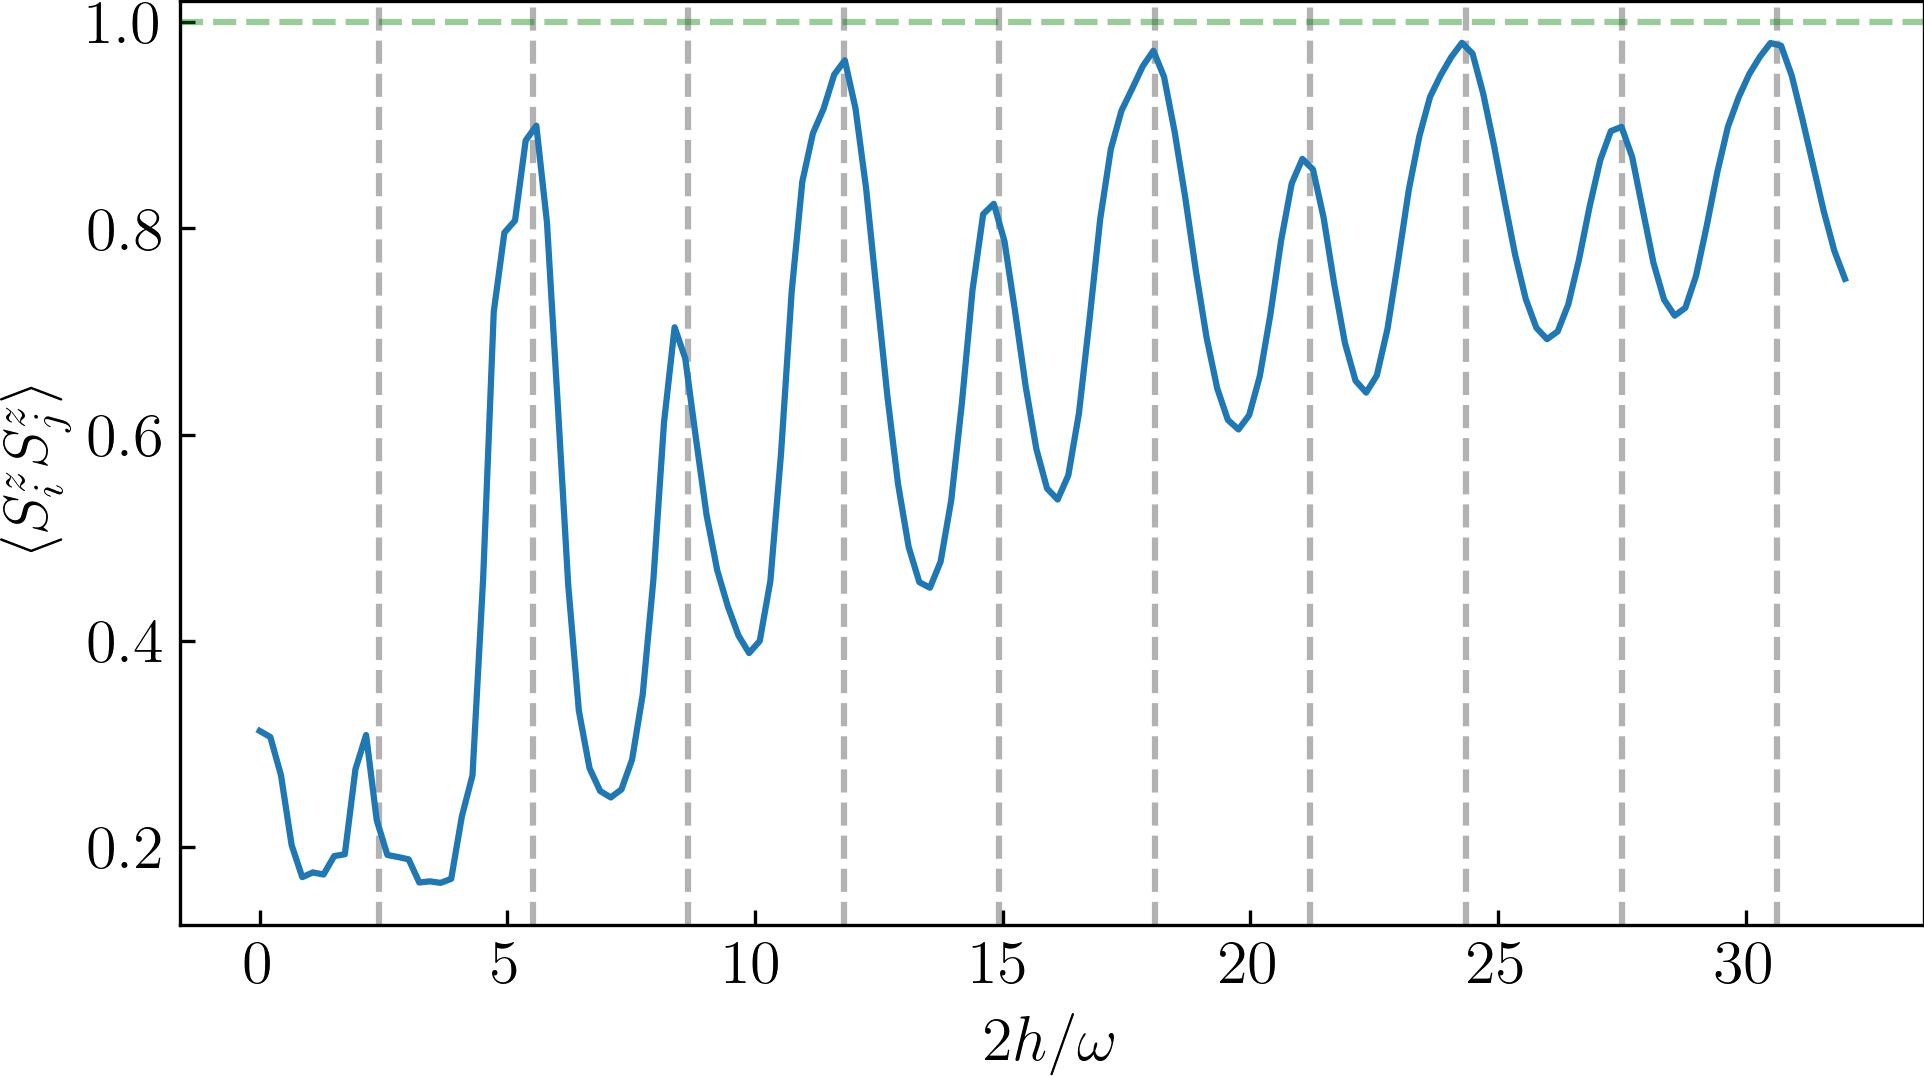
\includegraphics[width=8.5cm]{corrN8sz0sz3avg_onlynn_tfim_sx.jpeg}
				\caption{Temporal average of Spin-Spin correlation ($\expval{S^z_i S^z_j}$) for different $(2h/\omega)$, between two spins(i=0, j=3) of a 1D spin-1/2 chain consisting of eight spins denoting a TFIM with an additional longitudianl field($\sum_i\hat{\sigma}^x_i$).  The  vertical dashed lines are the roots of Bessel function($\mathcal{J}_0$). The spin correlation is suppressed at lower ($2h/\omega$) ratio, however it tends to attain unity at higher roots of $\mathcal{J}_0$.}
				\label{fig:TFIM_sx}
			\end{figure}
			
			We have numerically evolved the Hamiltonian $\hat{H}_{TFIM+S_x}(t)$ of Eq. \eqref{eq:tfim_sx1} to investigate the long-time averaged spin-spin correlation $\expval{S^z_i S^z_{j}}$ between two spins (site(i)=0, and site(j)=3) of a 1D spin chain consisting of eight spins (considering the periodic boundary condition).  $\expval{S^z_i S^z_{j}}$ is plotted for different values of the drive parameter ratio $(2h/\omega)$ corresponding to the constant drive frequency $\omega=90$. At lower values of $(2h/\omega)$, the time average of $\expval{S^z_i S^z_{j}}$ is found to be suppressed even at the resonance point (root of $\mathcal{J}_0$). As the ratio is found to rise gradually, the time average of $\expval{S^z_i S^z_{j}}$ is also found to rise to unity for all peaks. This corroborates the assertion that freezing is recovered at points corresponding to the higher roots of $\mathcal{J}_0$.
		}
		
		\item The referee says, \comment{``\textit{In the discussion of phase crossover from thermal to DMBL, increasing N in Fig 8 appears to push the regime of the local phase to a larger drive frequency. This seems to raise the same concerns associated with the stability of disorder-induced localization, as in whether one needs infinite disorder or infinite driving frequency to get a localization in the thermodynamic limit. Is this the case?}"}.
		
		\response{    	
			We thank the referee for the comment. We have extended our simulations to larger system sizes and have verified that this is indeed the case. Increasing $N$ pushes the crossover point further to larger values of $\omega$, thus requiring an infinite frequency at an infinite size. We have updated the corresponding figure (Fig.9 in revised manuscript), and have reported this in page 11 Section 4 par. 2.
		}
		\item The referee says, \comment{``\textit{Is the heating suppressed at points where the frequency meets the resonance condition? }"}.
		
		\response{
			We thank the referee for this comment. Although the concept of `heating' is inapplicable in the integrable TFIM case (as the system never thermalizes), the heating is, indeed, suppressed at the resonance condition for the long-range LMG model, provided the frequency is large enough to take the system out of the low-frequency regime. This can be seen in the standard deviation plots of the heating rate in figure 9 of the manuscript. There, the system is always kept at the resonance condition, but the deviation corresponds to the infinite temperature value for small frequencies, but increases as we traverse the crossover to the DMBL phase. Higher values arise due to integrable dynamics, and heating is suppressed since the IPR of the Floquet states is unity in that regime.}
		
		\item The referee says, \comment{``\textit{The discussion related to Fig. 9 could be improved, and it is not clear to me why the standard deviation of temporal fluctuations should vanish for thermalizing systems}"}.\\
		
		\response{ We thank the referee for pointing out the issue. We have improved that particular discussion. We have revised the discussion in Section IV, 3rd para., as well as improved the corresponding Fig.(10) in the revised manuscript. A more detailed explanation follows.
			
			
			The Hamiltonian for the LMG model,
			\begin{equation}
				\mathcal{H} = \frac{J}{2(N-1)}\sum_{i\neq j}\hat{\sigma}^z_i \hat{\sigma}^z_j +\Big[h_0 +h_1 \cos(\omega t)\Big] \sum_i \hat{\sigma}^x_i
			\end{equation}
			In the full Hilbert space, neglecting the dc part ($h_0$) for simplicity, the long-time average of the Hamiltonian in the lab frame is
			\begin{equation*}
			\bar{\mathcal{H}}	= {H}_0 \equiv \frac{J}{2(N-1)}\sum_{i\neq j}\hat{\sigma}^z_i \hat{\sigma}^z_j.
			\end{equation*}
			Squaring this term yields
			\begin{equation}
				\left({H_0}\right)^2 = \frac{J^2}{4(N-1)^2}\sum_{i\neq j, k \neq l} \hat{\sigma}^z_i \hat{\sigma}^z_j \hat{\sigma}^z_k \hat{\sigma}^z_l 
			\end{equation}
			The thermal variance at $T= \infty$ is given by $\displaystyle \sigma^2_{\infty} = \frac{\Tr[H^2_0]}{2^N}$. 
			Noting that ${H_0}$ is traceless, we only need the trace parts of $\left({H_0}^2\right)$ (the terms in the sums where $i=l, j=k,\;\&\;i=k, j=l$). Thus, we get
			\begin{align*}
				\sigma_\infty^2 =& \frac{J^2}{4(N-1)^2 2^N}\Tr[\sum_{i\neq j} \mathbbm{1}\otimes\mathbbm{1}\otimes \dots\hat{\sigma}^z_i \hat{\sigma}^z_i\dots\otimes \mathbbm{1} \otimes \dots \hat{\sigma}^z_j\hat{\sigma}^z_j \dots\otimes \mathbbm{1} \otimes\mathbbm{1}\otimes \dots]\\
				=& \frac{J^2}{4(N-1)^2}   \sum_{i\neq j} 1\\
				=& \frac{J^2}{4(N-1)^2} \frac{N(N+1)}{2}\\
				=& \frac{J^2}{8} \frac{N^2+N}{N^2-2N+1}.
			\end{align*}
			When $N\rightarrow \infty$, we have, by l'Hopital's rule,
			\begin{equation}
				\lim\limits_{N\rightarrow\infty}\sigma_\infty^2 = \frac{J^2}{8}.
				\label{eq:std_inf}
			\end{equation} 
			\begin{figure}[h!]
				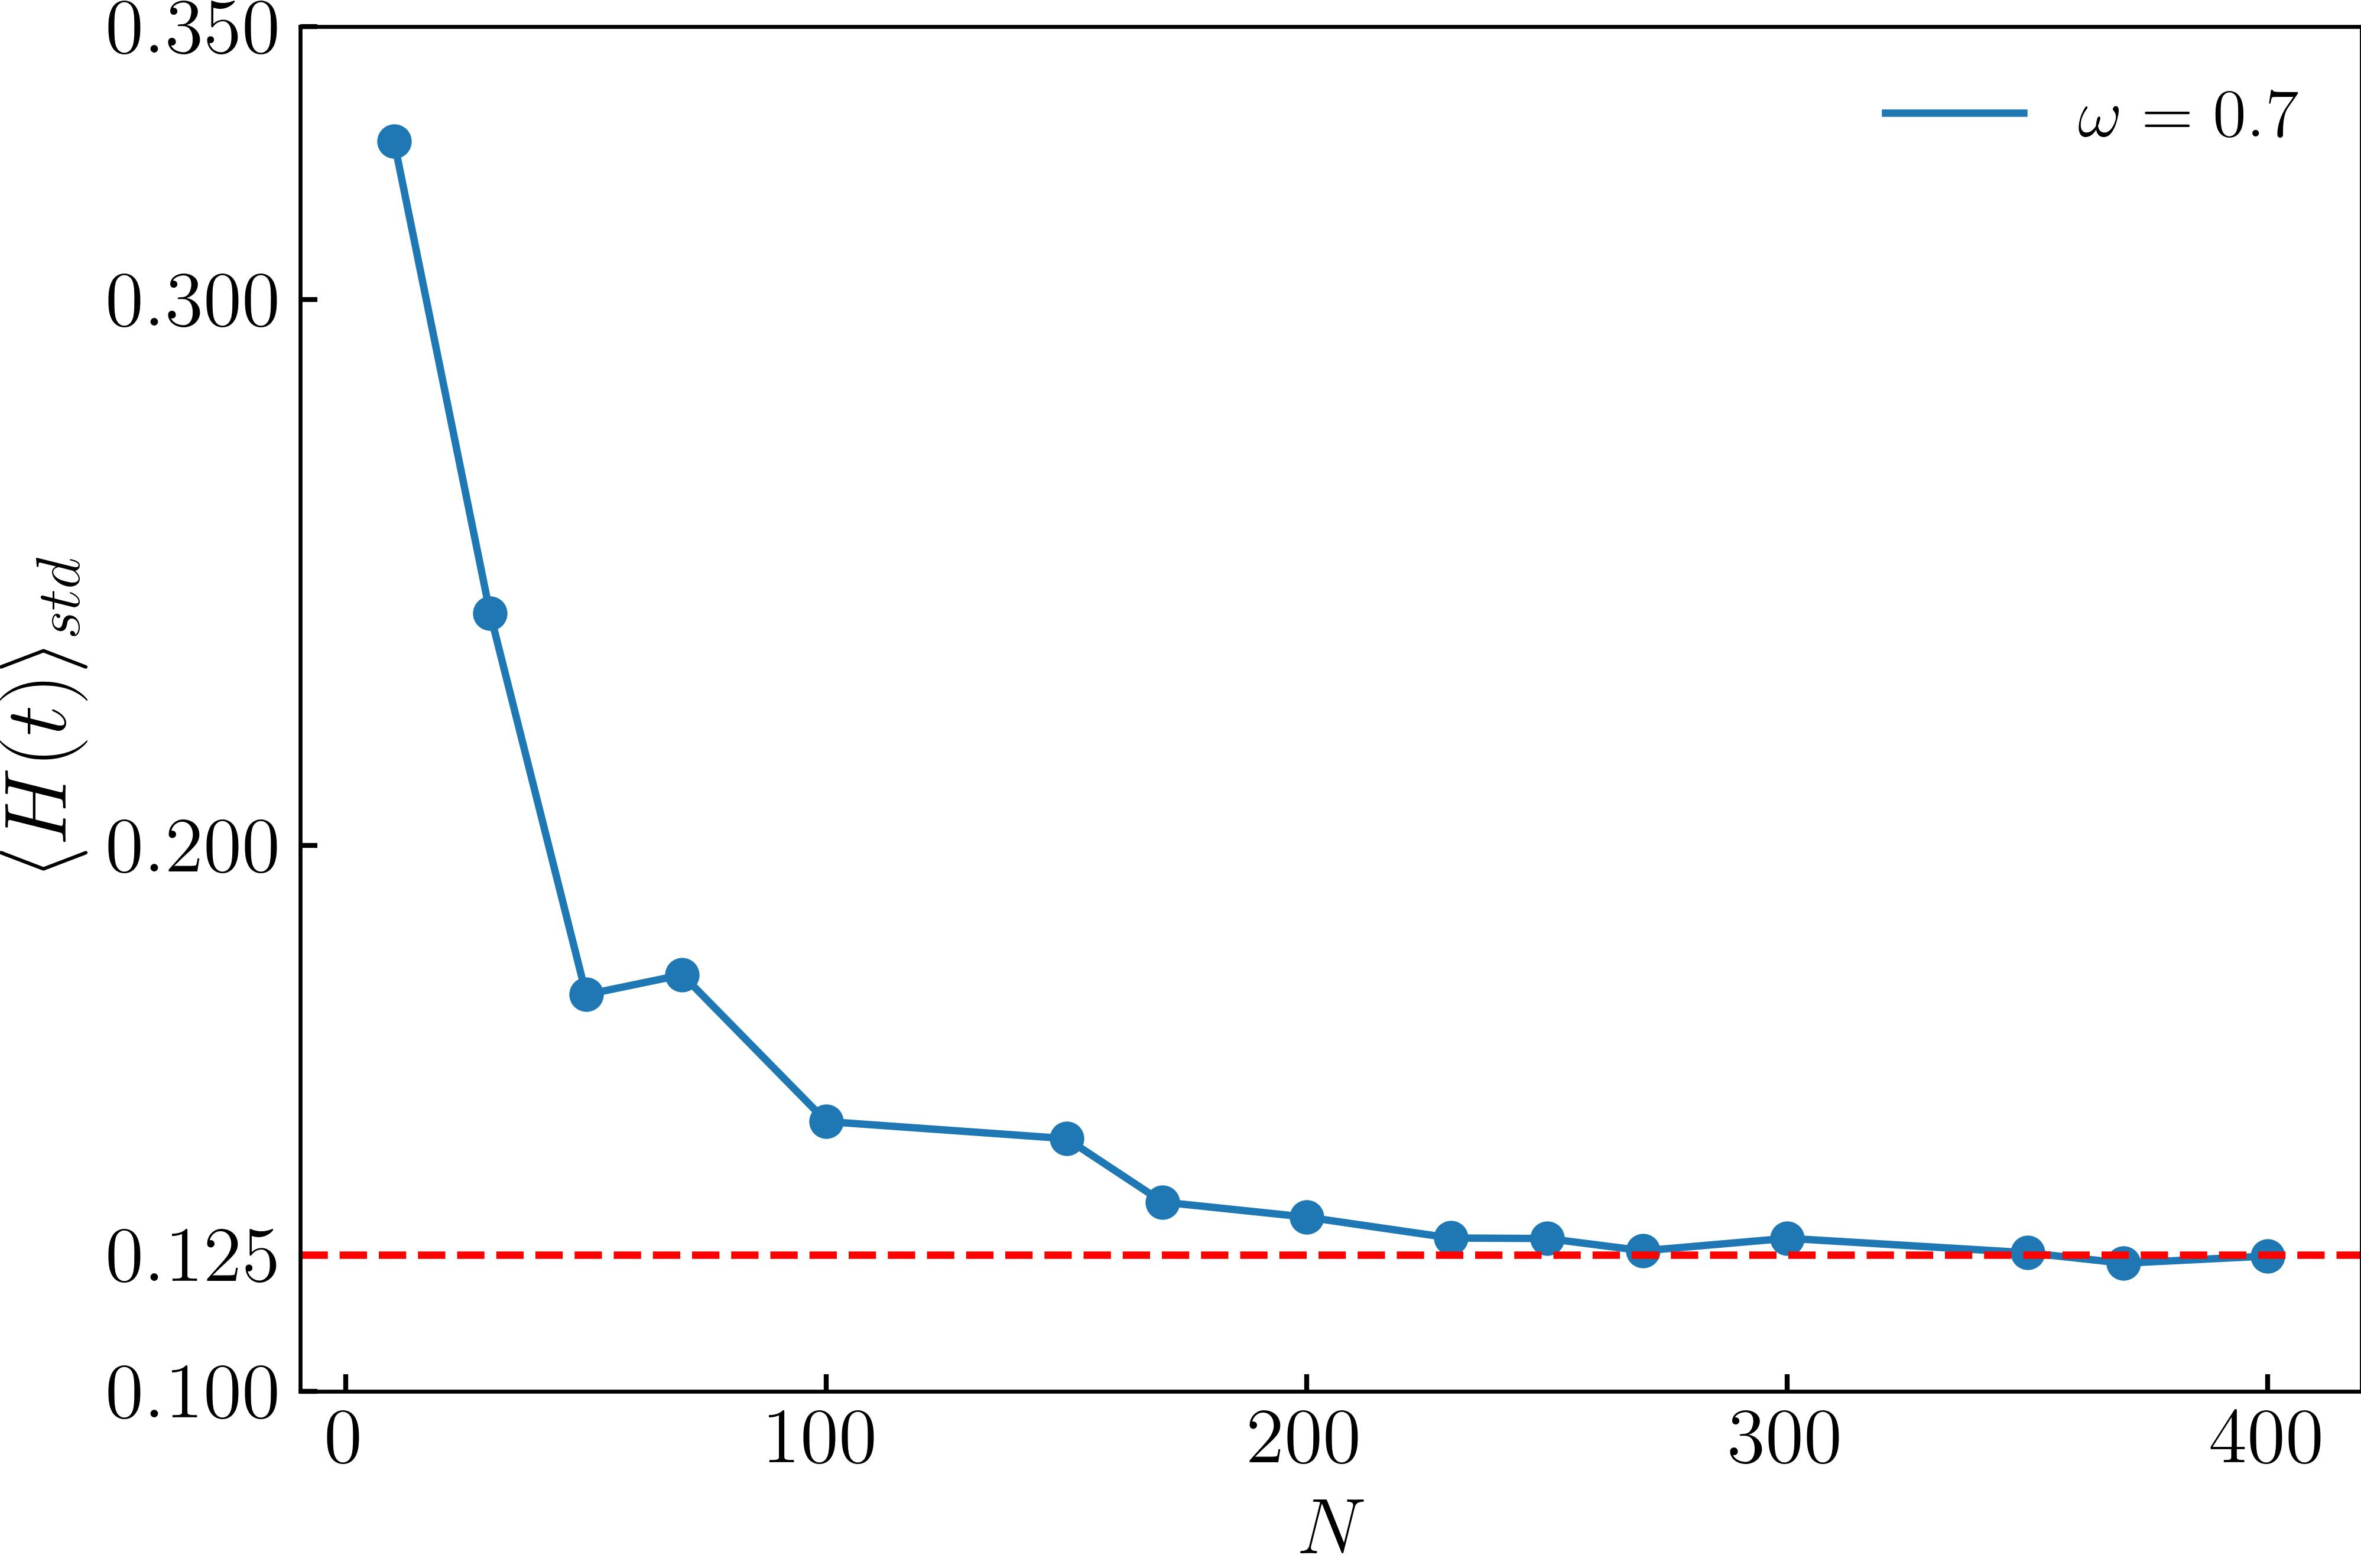
\includegraphics[width=8.5cm]{hbar_avg_std_w0p7.jpg}
				\caption{Variation of $\expval{H(t)}_{std}$ with system size(N) at small frequency $\omega=0.7$. $\expval{H(t)}_{std}$ is found to decrease as N increases and at thermodynamic limit it reaches 0.125.}
				\label{fig:std_N}
			\end{figure}
			For convenience, we had set $J=1$ in the manuscript. At low drive frequencies, we thus expect that $\expval{H(t)}_{std}$ will tend to this thermal value. Thus, $\sigma_\infty^2 = 0.125$. The numerical result in Fig.\ref{fig:std_N} supports the analytical results of Eq. \eqref{eq:std_inf}. We have updated the manuscript with a brief footnote summarizing this point, and added fig.~\ref{fig:std_N} as an inset.
		}
		
		
		\vskip 2cm
		\item The referee says, \comment{``\textit{In the conclusion, it is useful to comment on whether this method could be adapted (related to my point 2) to other generic models (say XXZ models)}"}.\\
		
		\response{
			We thank the referee for this suggestion. We have further elaborated on this issue in the manuscript. A detailed discussion follows.
			
			The generic XXZ model,
			\begin{equation*}
				H = \frac12 \left( \sum_{i=1} J \big(\hat{\sigma}^x_i \hat{\sigma}^x_{i+1} + \hat{\sigma}^y_i \hat{\sigma}^y_{i+1}\big) + \Delta  \hat{\sigma}^z_i \hat{\sigma}^z_{i+1} + h(t)  \hat{\sigma}^z_i\right).
				\label{eq:heisenberg_model}
			\end{equation*}
			We consider the drive, $h(t) = h \cos(\omega t)$. The unitary evolution operator $\displaystyle \hat{U}(t)$ is $\hat{U}(t)=\prod_{i} \exp \left(-i \frac{h}{2 \omega} \sin (\omega t) \hat{\sigma}_{i}^{z}\right)$. Now, the Hamiltonian, in the moving frame, is
			\begin{align}
				\tilde{H}(t)_{_{XXZ}}^{mov}= & \frac{1}{2} \exp \left(i \frac{h}{2 \omega} \sin (\omega t) \sum_{i} \hat{\sigma}_{i}^{z}\right)\left(\sum_{i} J \hat{\sigma}^x_i \hat{\sigma}^x_{i+1} + J \hat{\sigma}^y_i \hat{\sigma}^y_{i+1}+ \Delta  \hat{\sigma}^z_i \hat{\sigma}^z_{i+1}\right) \exp \left(-i \frac{h}{2 \omega} \sin (\omega t)\right)\nonumber\\
				= \frac12 \Bigg[& \underbrace{\exp \left(i \frac{h}{2 \omega} \sin (\omega t) \sum_{i} \hat{\sigma}_{i}^{z}\right)\left(\sum_{i} J \hat{\sigma}_{i}^{x} \hat{\sigma}_{i+1}^{x}\right) \exp \left(-i \frac{h}{2 \omega} \sin (\omega t) \sum_i\hat{\sigma}_{i}^{z}\right)}_{\mathrm{A}} \nonumber\\
				& +\underbrace{\exp \left(i \frac{h}{2 \omega} \sin (\omega t) \sum_{i} \hat{\sigma}_{i}^{z}\right)\left(\sum_{i} J \hat{\sigma}_{i}^{y} \hat{\sigma}_{i+1}^{y}\right) \exp \left(-i \frac{h}{2 \omega} \sin (\omega t) \sum_i\hat{\sigma}_{i}^{z}\right)}_{\mathrm{B}} \nonumber\\
				& +\underbrace{\Delta \left(\sum_{i}  \hat{\sigma}_{i}^{z} \hat{\sigma}_{i+1}^{z}\right)}_{\mathrm{C}}\Bigg]
				\label{eq:xxz1}
			\end{align}
			Here, we have split the RHS to three terms (A,B, and C). Now, defining $\zeta = \frac{h}{\omega}\sin(\omega t)$ we get simplifications for each of the three terms as follows.
			\begin{align}
				A &= \sum_{i} J \left[ \hat{\sigma}^x_i \hat{\sigma}^x_{i+1} \cos[2](\zeta) + \hat{\sigma}^y_i \hat{\sigma}^y_{i+1} \sin[2](\zeta)- \frac12\left(\hat{\sigma}^x_i \hat{\sigma}^y_{i+1} + \hat{\sigma}^y_i \hat{\sigma}^x_{i+1}\right)\sin(2\zeta)\right],
				\nonumber\\
				B &= \sum_{i} J \left[ \hat{\sigma}^x_i \hat{\sigma}^x_{i+1} \sin[2](\zeta) + \hat{\sigma}^y_i \hat{\sigma}^y_{i+1} \cos[2](\zeta)+ \frac12\left(\hat{\sigma}^x_i \hat{\sigma}^y_{i+1} + \hat{\sigma}^y_i \hat{\sigma}^x_{i+1}\right)\sin(2\zeta)\right],
				\label{eq:abmov}
			\end{align}
			Note that `C' doesn't change.
			
			Thus putting the values of $A, B$ \& $C$ in Eq.~\eqref{eq:xxz1} we get,
			\begin{equation}
			\tilde{H}(t)_{_{XXZ}}^{mov} = \frac12\sum_i\bigg[J\big(\hat{\sigma}^x_i\hat{\sigma}^x_{i+1} + \hat{\sigma}^y_i\hat{\sigma}^y_{i+1}\big) + \Delta\hat{\sigma}^z_i\hat{\sigma}^z_{i+1}\bigg]
			\label{eq:xxz_mov1}
			\end{equation}
		 We consider fermionic creation and annihilation operator, $\hat{\sigma}^+$ and $\hat{\sigma}^-$ respectively and transforming the moving frame Hamiltonian in their terms,
		\begin{align}
			H_{_{XXZ}}^{mov} =& \sum_i\Bigg[J\hat{\sigma}^+_i \hat{\sigma}^-_{i+1} + J\hat{\sigma}^-_i \hat{\sigma}^+_{i+1} + \frac{\Delta}{2} \hat{\sigma}^z_i \hat{\sigma}^z_{i+1}\Bigg],
			\label{eq:xxz_mov2}
		\end{align} 
		where, $\hat{\sigma}^+_i = 1/2(\hat{\sigma}^x_i + i\hat{\sigma}^y_i)$ and $\hat{\sigma}^-_i = 1/2(\hat{\sigma}^x_i - i\hat{\sigma}^y_i)$. The first two terms in the above Eqn.~\eqref{eq:xxz_mov2} annihilates a fully $z-$polarized state. However, if we populate the system with fully polarized state, which is one of the eigenstates of $\displaystyle \sum_i \hat{\sigma}^z_i \hat{\sigma}^z_{i+1}$, the contribution from $\displaystyle \sum_i \hat{\sigma}^z_i \hat{\sigma}^z_{i+1}$ gets the moving frame Hamiltonian frozen under periodic drive. However, if a longitudinal field $\sum_i \hat{\sigma}^x_i$ is augmented in XXZ model, then the dynamics of the system changes. It adds a single particle dynamics to the moving frame Hamiltonian. Thus, the Hamiltonian becomes
			\begin{equation*}
				H(t)_{XXZ + S_x} = \frac12 \left( \sum_{i=1} J \hat{\sigma}^x_i \hat{\sigma}^x_{i+1} +J  \hat{\sigma}^y_i \hat{\sigma}^y_{i+1} + \Delta \hat{\sigma}^z_i \hat{\sigma}^z_{i+1} + h\cos(\omega t) \hat{\sigma}^z_i + \hat{\sigma}^x_i\right).
				\label{eq:xxz_sx}
			\end{equation*}
			In order to move to the rotating frame, the transformation operator to be applied is $\displaystyle \hat{U}(t)$ is, $\hat{U}(t)=\prod_{i} \exp \left(-i \frac{h}{2 \omega} \sin (\omega t) \hat{\sigma}_{i}^{z}\right)$. The XXZ part of the Hamiltonian transforms in the same way as before.	The transformation + RWA approximation for the longitudinal field works out as follows. First, we define proper angular momenta $\displaystyle S^{\mu(=x,y,z)} = \frac12\sum_i \hat{\sigma}^\mu_i$, so that we can transform
			\begin{align*}
				\frac12 \sum_i \hat{\sigma}^x_i & \rightarrow\frac{1}{2} \exp \left(i \frac{h}{2 \omega} \sin (\omega t) \sum_{i} \hat{\sigma}_{i}^{z}\right)\left(\sum_{i} \hat{\sigma}_{i}^{x}\right) \exp \left(-i \frac{h}{2 \omega} \sin (\omega t) \hat{\sigma}_{i}^{z}\right) \\
				& =\left(e^{i 2 \eta S^{z}} S^{x} e^{-i 2 \eta S^{z}}\right),
			\end{align*}
			where we have used the Baker-Campbell-Hausdorff formula, together with the canonical angular momentum commutation relations. Applying the Jacobi Anger expansion again, recalling that $\eta=\frac{h}{2 \omega} \sin (\omega t)$ and taking the RWA that keeps only $0^{th}$ order terms in the expansion, yields
			\begin{equation}
				\Big(\frac12 \sum_i \hat{\sigma}^x_i\Big) \rightarrow \left(S^{x} \cos (2 \eta)-S^{y} \sin (2 \eta)\right)^{RWA} \approx \mathcal{J}_{0}\left(\frac{h}{\omega}\right) S^{x} = \mathcal{J}_{0}\left(\frac{h}{\omega}\right)\frac12\sum_i\hat{\sigma}^x_i.
			\end{equation}
		Thus the full Hamiltonian after RWA becomes,
		\begin{equation}
		\hat{H}_{_{XXZ + S_x}} = H^{mov}_{xxz} + \frac12 \mathcal{J}_{0}\left(\frac{h}{\omega}\right)\sum_i\hat{\sigma}^x_i
		\end{equation}
		If the drive parameters $h$ and $\omega$ are adjusted in such a way that the ratio $h/\omega$ is one of the root of Bessel function $\mathcal{J}_0$ then $\hat{H}_{_{XXZ + S_x}}$ reduces to $\hat{H}_{xxz}^{mov}$ which is frozen for all $h/\omega$.
				
	\begin{figure}[t!]
		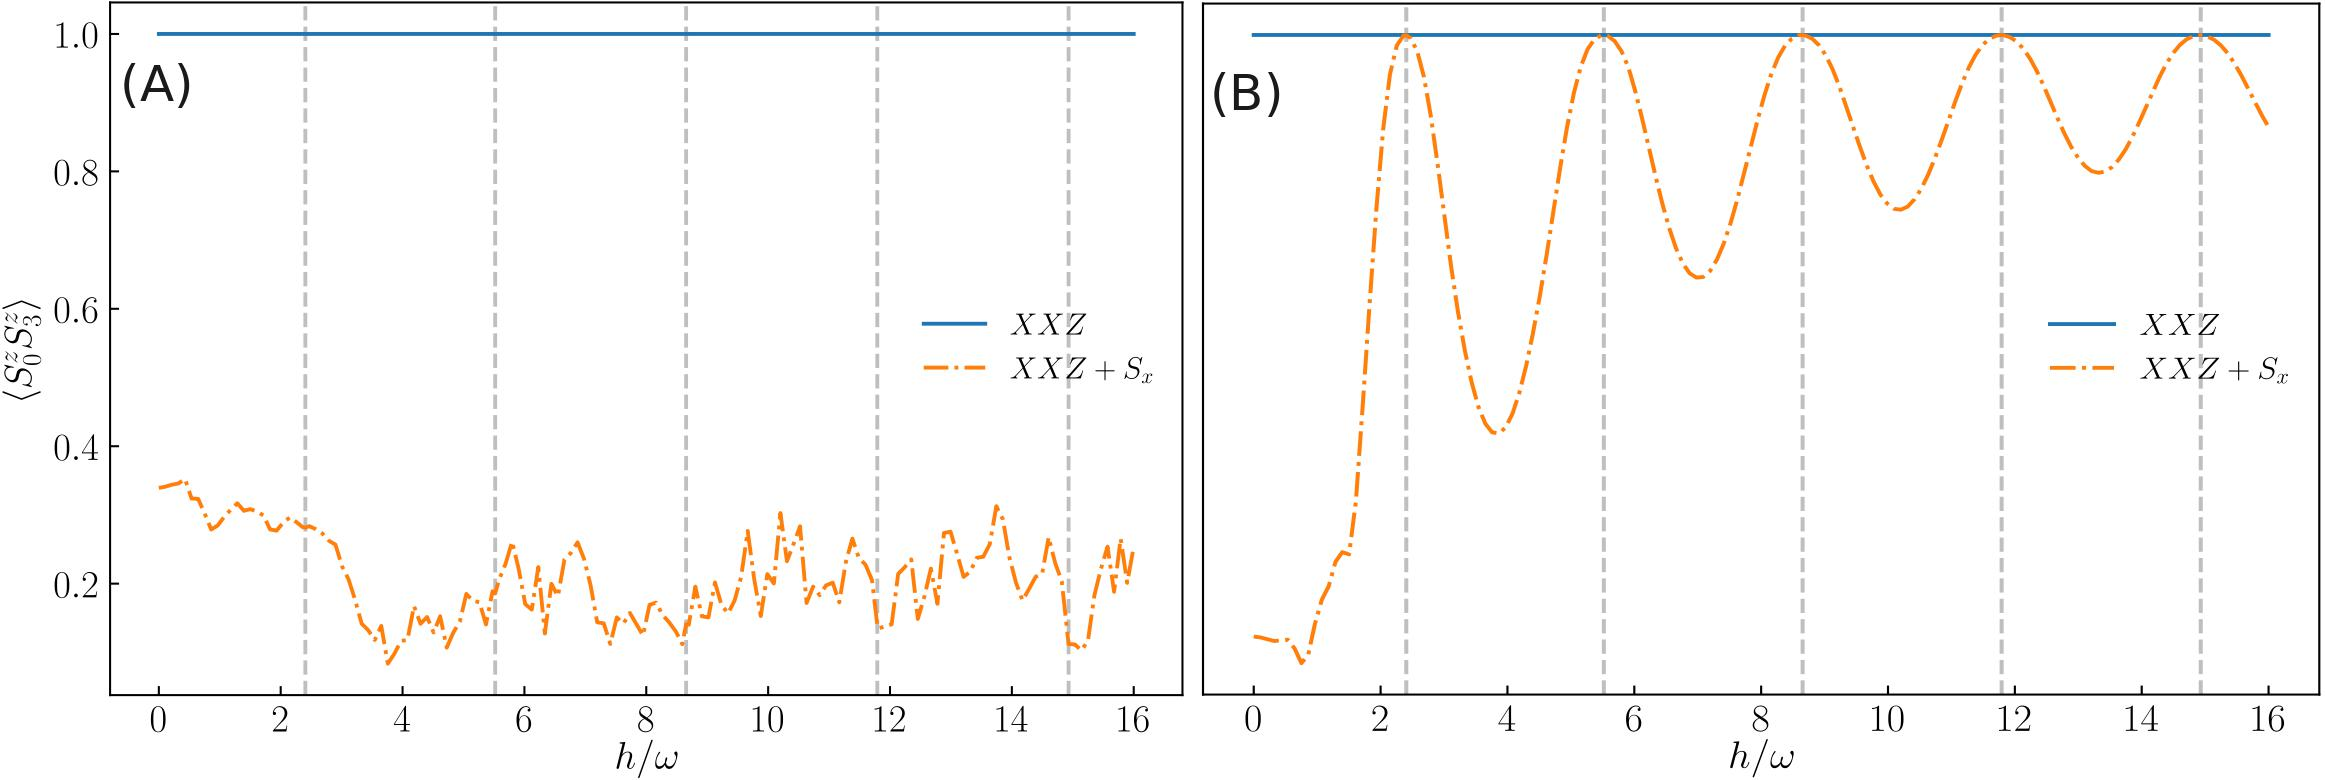
\includegraphics[height=5cm]{xxz_sx_low_high_fr.jpeg}
		\caption{The temporal average of the spin-spin correlation $\expval{S^z_0 S^z_3}$ is shown for various $(2h/\omega)$ values. The correlation is measured between two spins (i= 0 and j = 3) in a 1D spin-1/2 chain consisting of eight spins, representing an XXZ model and for additional longitudinal field $S_x$ field augmented to it. The frequency is adjusted to $\omega=0.5$ (left panel-A) and $\omega=90$ (right panel-B), with an anisotropy value of $\Delta=1.5$. The vertical dashed lines represent the roots of the Bessel function ($\mathcal{J}_0$). All $h/\omega$ exhibit a spin correlation of unity for the XXZ model, indicating drive-independent freezing. Though in the case of the introduction of additional integrability-breaking terms in the XXZ model, freezing occurs only when the drive frequency is high and the drive parameter $h/\omega$ is one of the roots of $\mathcal{J}_0$ as shown in Panel-B. However, at low frequency $\omega=0.5$, the system exhibits thermal behavior.}
		\label{fig:xxz}
	\end{figure}

	We conducted a simulation of the Hamiltonian described in Eq.~\eqref{eq:heisenberg_model} to compute the time-averaged spin-spin correlation $\expval{S^z_0 S^z_3}$ using numerical methods. The system is set with a value of $N=8$, a drive frequency of $\omega=90$, and correlation sites at $i=0$ and $3$. The spin correlation $\expval{S^z_0 S^z_3}$ is determined to be consistently unity for all $h/\omega$, as shown in Fig.~\ref{fig:xxz}. This supports the analytical expression which suggests the XXZ model becomes localized when a periodically driven field is present, regardless of the drive parameters. Although if an additional symmetry breaking term is introduced a freezing is possible only at specific system parameters as can be seen in Fig.~\ref{fig:xxz}. So a pure XXZ can not be chosen for our method, however additional $\sum_i \hat{\sigma}^x_{i}$ term will manipulate the system to exhibit creation or destruction of freezing.
	}
	\end{enumerate}
	
	\vskip 1cm 
	\noindent \textbf{Summary of important changes to the  manuscript}
	\begin{enumerate}
		\item We have discussed the novelty of our work in the Introduction, para. 6.
		\item We have added references in support of FETH in Section 1 para. 3 (page 3).
		\item We have improved the discussion on how freezing manifests in more general spin systems, particularly with integrability breaking terms and the XXZ case, in Section 1 paras 4 \& 5 (pages 4\& 5). Additionally, we have inserted a new Fig. (1) in support of our conclusions (all other figures have been renamed accordingly).
		\item We have improved the labeling of Figs. 2 and 8, and updated the respective captions.
		\item We have discussed the size scaling of crossover in Section IV para 2 (page 11).
		\item We have improved Fig. 9 by adding an inset figure describing the dependency of the crossover frequency on system size.
		\item We have improved Fig. 10 by adding an inset that shows a plot of the standard deviation of heating rate $\expval{H}_{std}$ at low frequency range as well. We have also included a brief discussion on this in the caption.
	\end{enumerate}
	
	\bibliography{dmbl_refs}
	
	
\end{document}